\documentclass{beamer}
\usetheme[hideothersubsections]{UNLTheme}
\usepackage{graphics}
\usepackage{setspace}
\usepackage{graphicx}
\usepackage{hyperref}
\usepackage{ragged2e}
\usepackage[utf8]{inputenc}
\usepackage[english]{babel}
%\usepackage{enumitem}
%\usepackage[usenames]{xcolor}
%\usepackage[svgnames]{color}
\usepackage{color}
\usepackage{verbatim}
%\usepackage{multicol}
\usepackage{epstopdf}
% Alogorithm related packages start here
%\usepackage[lined]{algorithm2e}
%\usepackage{algorithmic}
\usepackage{makecell}
\usepackage{algorithm}
%\usepackage{algpseudocode}
\usepackage{gensymb}
\usepackage{algorithmic}
\usepackage{multirow}
%\floatname{algorithm}{Procedure}
\renewcommand{\algorithmicrequire}{\textbf{Input:}}
\renewcommand{\algorithmicensure}{\textbf{Output:}}
%\usepackage[noend]{algpseudocode}
%\textwidth	=165.mm
% Alogorithm specific package end here
\usepackage{multirow}
\usepackage{array,booktabs,calc,tabularx}
\useoutertheme{infolines}
\useinnertheme{default}
\usecolortheme{default}
\setbeamertemplate{headline}{}
\setbeamertemplate{frametitle}[default][center]
%% for References (Continous slides)
\setbeamertemplate{frametitle continuation}[from second][... Contd.]
% \usepackage{algorithm}
% \usepackage[noend]{algpseudocode}

\newcommand{\bodyfont}{\small}
\newcommand{\tabfont}{\scriptsize}
\newcommand{\rowgap}{\addlinespace[4pt]}
% --- node-type colours for the SCM graph legend (match scm_graph.png) ---
\definecolor{nS}{HTML}{4C72B0}\definecolor{nM}{HTML}{55A868}\definecolor{nP}{HTML}{DD8452}
\definecolor{nD}{HTML}{8172B3}\definecolor{nR}{HTML}{C44E52}\definecolor{nO}{HTML}{CCB974}
\newcommand{\nodedot}[1]{\textcolor{#1}{\large$\bullet$}}


% --- YELLOW block: gold header, RGB(223,165,15); cream body, RGB(253,246,227) ---
\definecolor{coepyellow}{RGB}{223,165,15}
\definecolor{coepcream}{RGB}{253,246,227}
\newenvironment{yellowblock}[1]{%
  \setbeamercolor{block title}{bg=coepyellow, fg=black}%
  \setbeamercolor{block body}{bg=coepcream, fg=black}%
  \begin{block}{#1}}%
  {\end{block}}

\title[COEP Technological University, Pune]{Quantum GNN for Supplier Procurement Risk  Analysis}

%\vspace{1.5cm}
%\begin{columns}[8cm]
%\column{4cm}
%\hspace{0.05cm}

\author[MIS No 712522002 - Aditya Jagtap ]{}

{ }
%\institute[]{Department of Computer Engineering \& IT\\College Of Engineering, Pune\\
%\vspace{0.5 cm} \textbf {\textcolor[rgb]{0.6,0.0,0.0}{Doctoral Committee Meeting}}}

%\subject{Computational Sciences}
%First Seminar Talk
\begin{document}
\begin{frame}
\vspace{-0.5cm}
\begin{center}M. Tech. Dissertation Stage I - Mid Sem Exam\\Presentation on\end{center}
\vspace{-1cm}
\titlepage
\vspace{-0.5cm}
\begin{tabular}{cp{1.8cm}l}
  \textcolor[rgb]{0.6,0.0,0.0}{Presented by} & &
  \ \ \ \ \ \ \ \ \ \ \ \ \ \ \ \ \textcolor[rgb]{0.6,0.0,0.0}{Project Guide} \\
  Aditya Jagtap & & \ \ \ \ \ \ \ \ \ \ \ \ \ \ \ \ Dr. Amit D. Joshi \\ \newline712522002
\end{tabular}
\vspace{-0.5cm}
\begin{center}
  \begin{figure}[!t]
    
\includegraphics[scale=0.075]{COEP_Tech_University_Logo.jpg}
  \end{figure}
  \textcolor[rgb]{0.6,0.0,0.0}{Department of Computer Science and Engineering \\
  COEP Technological University (COEP Tech), Pune \\ September - 2026}
  \vspace{4mm}
\end{center}
\vspace{-1cm}
\end{frame}


\begin{frame}
\frametitle{Data Sheet}
\vspace{-2em}
\begin{center}
\large
\begin{tabular}{@{}p{3.2cm}@{\hspace{1.2em}}p{7.5cm}@{}}
\textbf{Name:}       & Aditya Jagtap \\[1em]
\textbf{MIS:}        & 712522002 \\[1em]
\textbf{Degree:}     & M.Tech (2025--2027) \\[1em]
\textbf{Branch:}     & Computer Engineering \\[1em]
\textbf{Department:} & Computer Science and Engineering,\newline
                       COEP Technological University Pune
\end{tabular}
\end{center}
\end{frame}

%-------------------------------------------------


\begin{frame}
\frametitle{Contents}
\bodyfont
\tableofcontents
\end{frame}
%------------------------------------------------

\section{Introduction}
%------------------------------------------------

\begin{frame}
\frametitle{Introduction}
\small
\begin{columns}[T]
\column{0.47\textwidth}
\begin{itemize}
  \item \textbf{Procurement:} sourcing materials from external suppliers so
        production can continue
  \vspace{0.3em}
  \item A supply chain is a \textbf{network}; a problem at one node
        \textbf{propagates along it}
  \vspace{0.3em}
  \item \textbf{Risk assessment:} predict which suppliers are likely to be
        disrupted, and how severely
  \vspace{0.3em}
  \item Hard: disruptions are \textbf{rare} (class imbalance) and
        \textbf{severe} events differ from normal history
\end{itemize}
\column{0.51\textwidth}
\centering
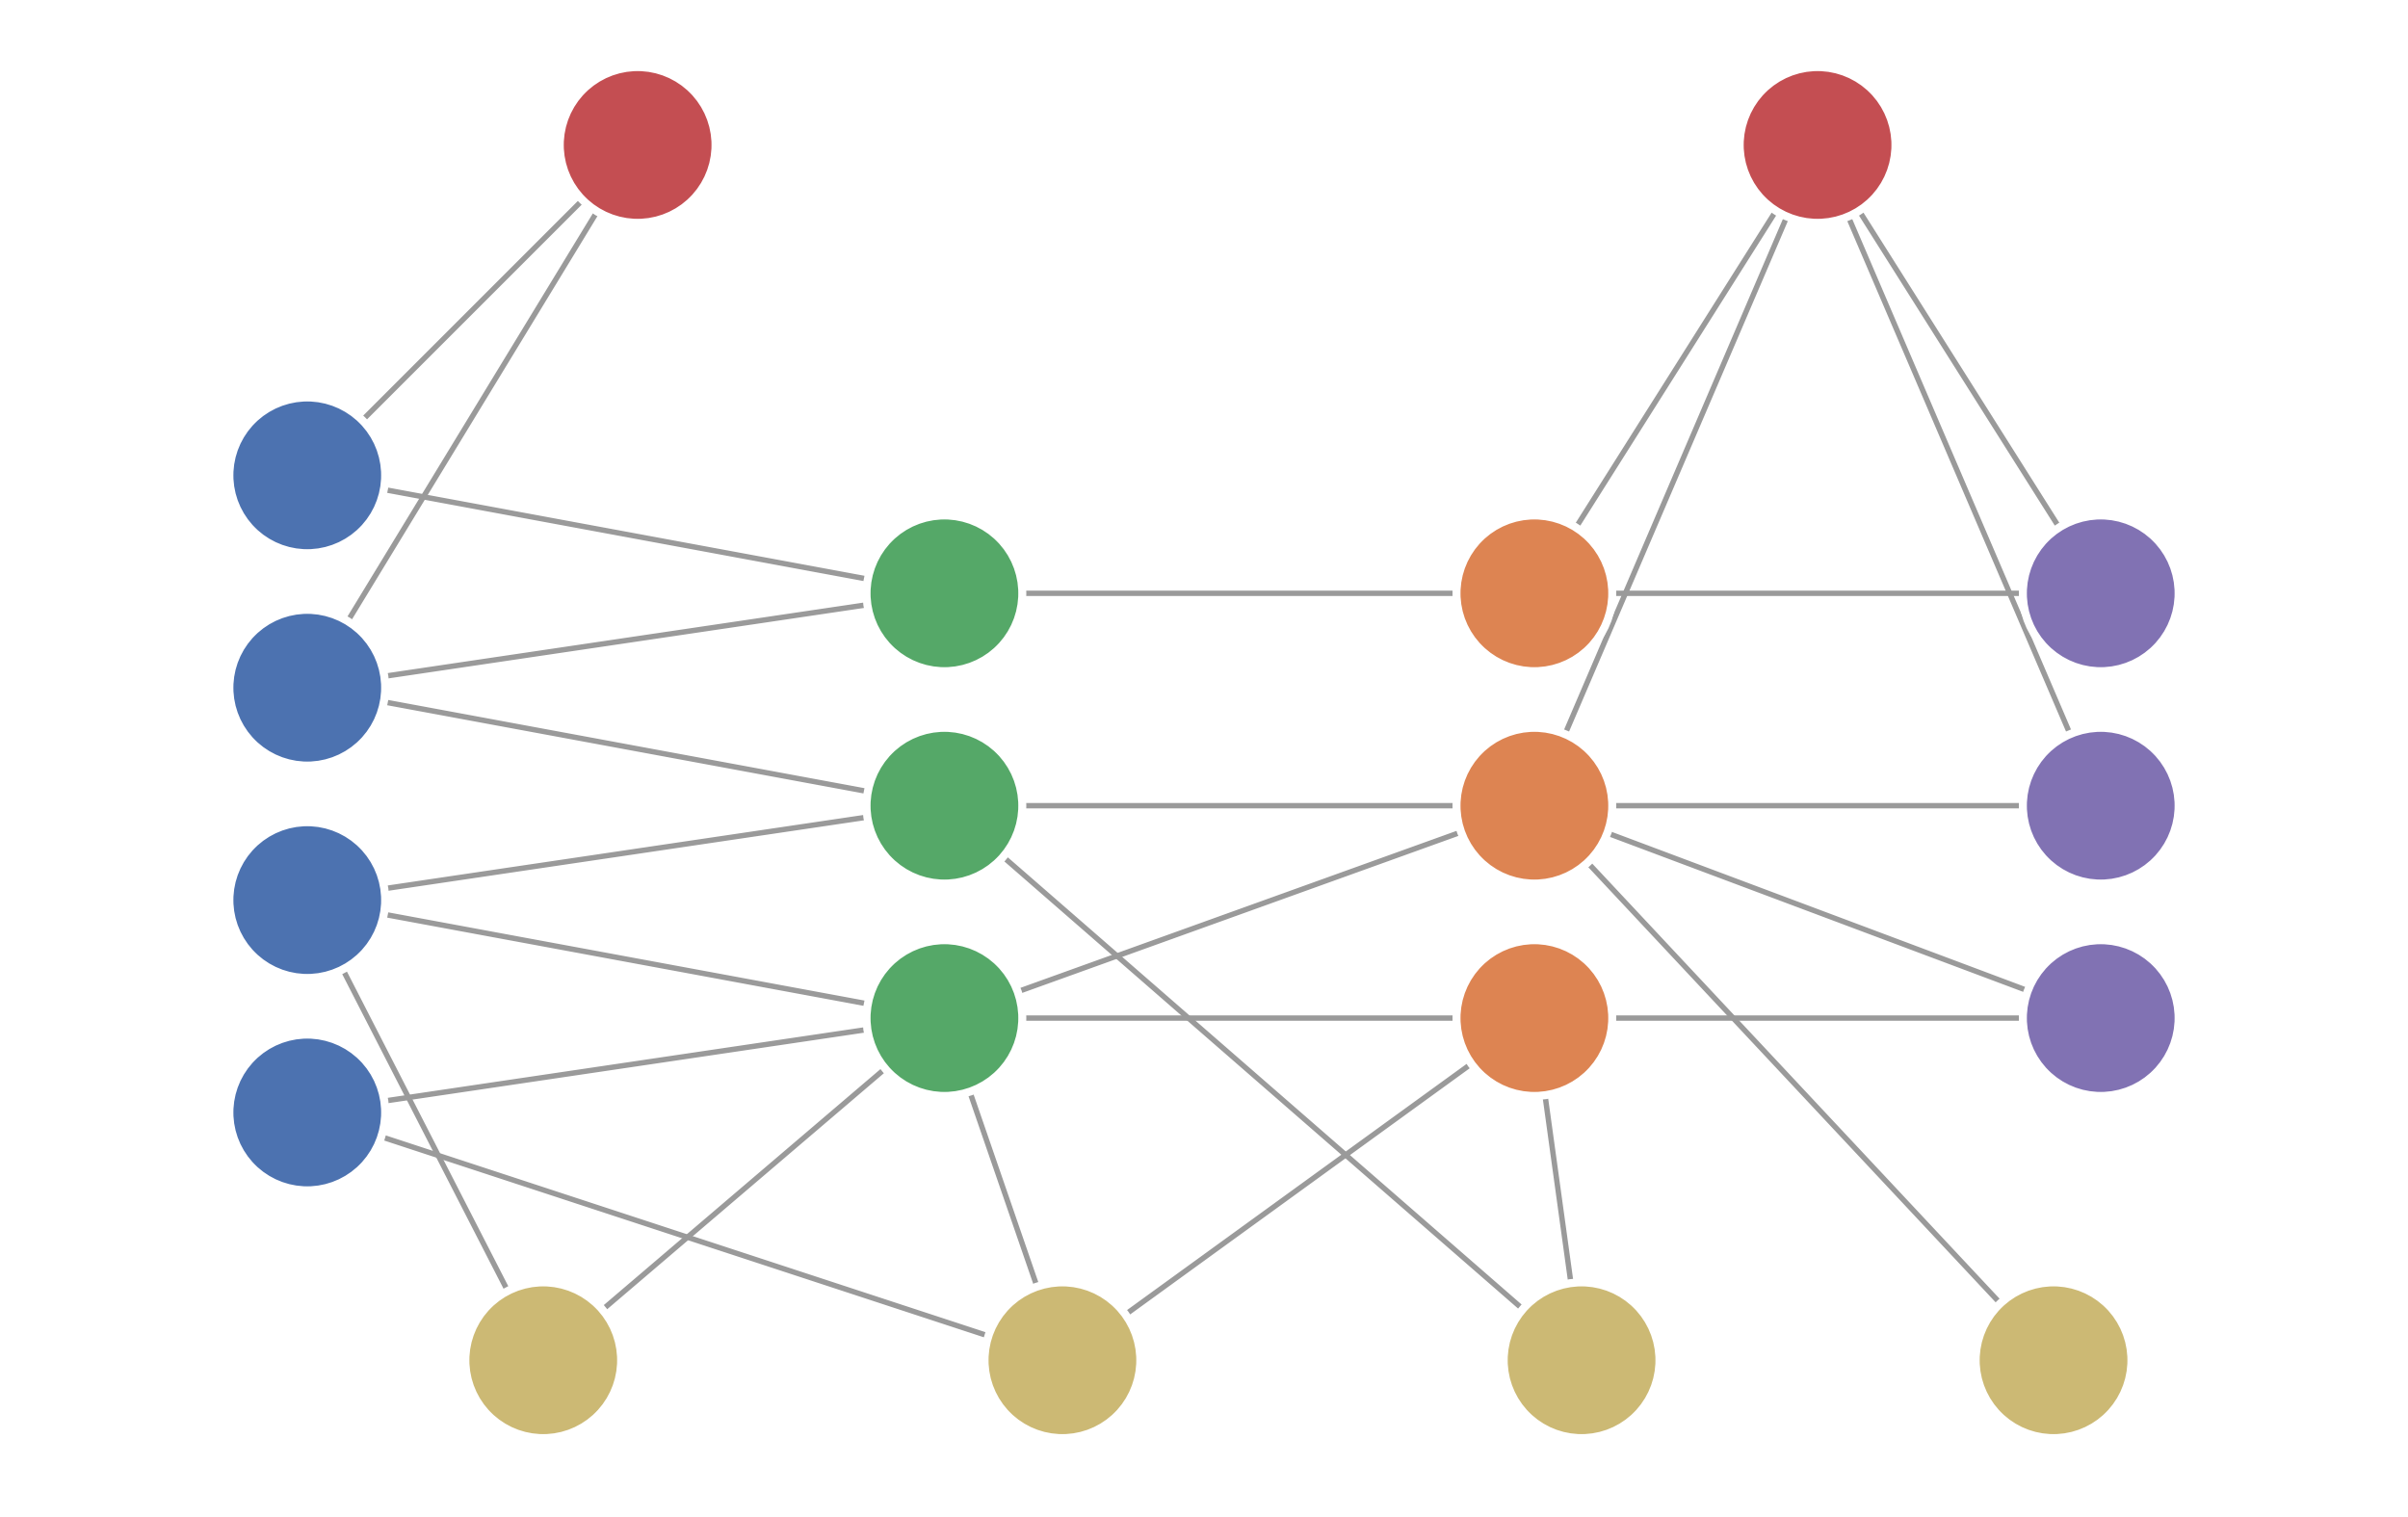
\includegraphics[width=\linewidth]{scm_graph.png}

{\tiny \nodedot{nS} Supplier (300)\quad \nodedot{nM} Material (100)\quad \nodedot{nP} Plant (50)\\
\nodedot{nD} Product (200)\quad \nodedot{nR} Region (20)\quad \nodedot{nO} Procurement order (2,000)\\[2pt]
Illustrative subgraph; full graph: 2,670 nodes, 7,675 edges}
\end{columns}
\end{frame}

%------------------------------------------------

\begin{frame}
\frametitle{Introduction Contd...}
\bodyfont
\begin{itemize}
  \item \textbf{GNN:} each node builds an embedding by aggregating its
        neighbours' information. \textbf{GraphSAGE} does this by sampling
        neighbours, so it scales
  \vspace{0.4em}
  \item For risk: suppliers are nodes, dependencies are edges, output is a
        \textbf{risk score per supplier}
  \vspace{0.4em}
  \item Classical limits: \textbf{over-smoothing} and \textbf{over-squashing}
  \vspace{0.4em}
  \item \textbf{QGNN:} a variational quantum circuit replaces part of the model.
        Thought to help (hypotheses we test):
  \begin{itemize}
    \item Encoding into a \textbf{high-dimensional Hilbert space}
    \item \textbf{Entanglement} models feature correlations compactly
    \item Very few parameters, suited to small data and rare events
  \end{itemize}
  \vspace{0.4em}
  \item \textbf{Our design:} a small VQC head on a \textbf{frozen GraphSAGE
        embedding}, as a controlled comparison with classical GraphSAGE ---
        not a quantum-advantage claim
\end{itemize}
\end{frame}

%%------------------------------------------------
\section{Literature Review}
\begin{frame}[t,shrink=12]
\frametitle{Literature Review}
\tabfont
\centering
\begin{tabularx}{\linewidth}{@{}>{\raggedright\arraybackslash}p{0.6cm}
                               >{\raggedright\arraybackslash}p{2.2cm}
                               >{\raggedright\arraybackslash}X
                               >{\raggedright\arraybackslash}X@{}}
\multicolumn{4}{@{}c@{}}{\textbf{Table 1: Literature Survey}} \\
\toprule
\textbf{Ref} & \textbf{Author (Year)} & \textbf{Focus / Method} & \textbf{Limitation} \\
\midrule
{[1]} & Fareed (2026) &
Classical ML for supplier risk prediction and resilience scoring &
Preprint, not peer-reviewed; purely classical, no quantum baseline \\ \rowgap

[2] & Ziaria et al. (2026) &
ML-based supplier evaluation; sustainable supplier selection and delay-risk framework &
Classical ML only; no graph structure or quantum component \\ \rowgap

[3] & Rahman \& Nguyen (2026) &
QCNN survey; entanglement-based correlation learning &
Survey only; no supply-chain or graph evaluation \\ \rowgap

[4] & Lamichhane \& Rawat (2025) &
Survey of QML: advances, challenges, perspectives &
Survey only; no empirical evaluation on any domain task \\ \rowgap

[5] & Larbi et al. (2025) &
Dual ML models for IoT component failure and parts demand &
Classical ML only; no quantum formulation \\
\bottomrule
\end{tabularx}
\end{frame}
%%------------------------------------------------
\begin{frame}[t,shrink=12]
\frametitle{Literature Survey}
\tabfont
\centering
\begin{tabularx}{\linewidth}{@{}>{\raggedright\arraybackslash}p{0.6cm}
                               >{\raggedright\arraybackslash}p{2.2cm}
                               >{\raggedright\arraybackslash}X
                               >{\raggedright\arraybackslash}X@{}}
\multicolumn{4}{@{}c@{}}{\textbf{Table 1: Literature Survey (Contd.)}} \\
\toprule
\textbf{Ref} & \textbf{Author (Year)} & \textbf{Focus / Method} & \textbf{Limitation} \\
\midrule
{[6]} & Innan et al. (2024) &
QGNN with VQC for credit-card fraud detection &
Simulator only; 6 qubits; heavy undersampling; $\approx$3\% gain over classical GNN \\ \rowgap

[7] & Tudisco et al. (2024) &
VQC classifier on real bank transaction data &
Dataset reduced in size and features via PCA due to NISQ limits; scalability unproven \\ \rowgap

[8] & Soni et al. (2024) &
Survey of quantum optimization in supply chain management and logistics &
Survey only; no learned risk-prediction model \\ \rowgap

[9] & Jiang, Shen \& Liu (2022) &
Quantum inventory model; supply-chain structures suited to quantum methods &
Inventory setting; no learned risk prediction or GNN \\ \rowgap

[10] & Yadav (2021) &
Survey of GCN/GAT risk propagation; GNNs model multi-hop supply-chain dependencies &
Survey only; classical GNNs, no quantum formulation \\
\bottomrule
\end{tabularx}
\end{frame}
%%------------------------------------------------
\section[Motivation]{Motivation and Need}
\begin{frame}[shrink=6]
\frametitle{Motivation and Need for Study}
\bodyfont
\begin{itemize}
  \item \textbf{Same structural problem as fraud:} rare, high-impact events in a
        relational network with extreme class imbalance --- the setting where
        QGNN and VQC work has been reported [6, 7]
  \vspace{0.4em}
  \item \textbf{Supplier networks are natively graphs:} suppliers, hubs and
        raw-material sources as nodes; dependency and material flow as edges
  \vspace{0.4em}
  \item \textbf{Classical GNNs struggle where procurement risk lives:}
        over-smoothing flattens embeddings at depth, over-squashing bottlenecks
        multi-hop signal
  \vspace{0.4em}
  \item \textbf{Gap in the surveyed work:}
  \begin{itemize}
    \item Supplier-risk studies are purely classical [1, 2, 5]
    \item Quantum studies target finance, are surveys, or address inventory [3, 4, 6--9]
    \item No QGNN applied to supplier procurement risk
  \end{itemize}
  \vspace{0.4em}
  \item \textbf{Need:} a \textbf{controlled comparison} against a classical
        GraphSAGE baseline, so the outcome is defensible either way
\end{itemize}
\end{frame}
%----------------------------------------------
%%-----------------------------------------------
\section{Problem Statement}
\begin{frame}
\frametitle{Problem Statement}
\bodyfont
\vspace{1em}
\begin{yellowblock}{Problem statement}
Comparative Study of Supplier Procurement Risk Analysis using GNN in
Classical and Quantum Computing Environments
\end{yellowblock}
\vspace{0.8em}
To investigate whether a \textbf{hybrid quantum-classical head}, a small
variational quantum circuit reading a frozen GraphSAGE supplier embedding, can
match or exceed a \textbf{classical GraphSAGE} baseline for
\textbf{supplier disruption-risk prediction}, and to identify which
architectural and training factors govern its behavior.
\end{frame}
%---------------------------------------------
%%--------------------------------------------
\section[Objectives]{Objectives}
\begin{frame}
\frametitle{Objectives}
\bodyfont
\begin{enumerate}
  \item \textbf{Formulate} supplier procurement risk as a node-level
        prediction task on a supply-chain graph
  \vspace{0.6em}
  \item \textbf{Implement} a classical GraphSAGE baseline for supplier
        disruption-risk prediction
  \vspace{0.6em}
  \item \textbf{Implement} a hybrid QGNN: a variational quantum circuit head
        on the frozen GraphSAGE embedding
  \vspace{0.6em}
  \item \textbf{Compare} the classical and quantum models under identical
        data, splits and metrics
  \vspace{0.6em}
  \item \textbf{Analyze} which design factors (encoding, qubits, depth)
        affect the hybrid model's behavior
\end{enumerate}
\end{frame}
%----------------------------------------------

\section{SRS}
\begin{frame}[t,shrink=14]
\frametitle{Software Requirements Specification}
\tabfont
\centering
\begin{tabularx}{\linewidth}{@{}>{\raggedright\arraybackslash}p{2.6cm}
                               >{\raggedright\arraybackslash}X@{}}
\multicolumn{2}{@{}c@{}}{\textbf{Table 2: Functional and Non-Functional Requirements}} \\
\toprule
\textbf{Requirement} & \textbf{Description} \\
\midrule
\multicolumn{2}{@{}l}{\textit{Functional}} \\ \rowgap
Data ingestion and graph construction &
Load the synthetic supplier dataset and build a heterogeneous supply-chain
graph (6 node types, 9 relation types) \\ \rowgap
Feature encoding &
Encode static and time-varying supplier attributes as node features \\ \rowgap
Hybrid risk model &
GraphSAGE encoder with a VQC head producing a supplier disruption-risk score \\ \rowgap
Disruption simulation &
Black-swan events simulated over 104 periods (about 2 years, weekly) \\ \rowgap
Evaluation and reporting &
PR-AUC and related metrics on temporal and severity splits, with tables and figures \\
\midrule
\multicolumn{2}{@{}l}{\textit{Non-functional}} \\ \rowgap
Fair comparison &
Classical and quantum models share the same data, splits and metrics \\ \rowgap
Reproducibility &
Fixed random seeds and saved experiment artifacts \\ \rowgap
Scalability &
Pipeline designed for larger graphs (currently 2,670 nodes, 7,675 edges) \\
\bottomrule
\end{tabularx}
\end{frame}

%------------------------------------------------

\begin{frame}[t]
\frametitle{SRS Contd...: Technology Stack}
\tabfont
\centering
\begin{tabularx}{\linewidth}{@{}>{\raggedright\arraybackslash}p{3.4cm}
                               >{\raggedright\arraybackslash}X@{}}
\multicolumn{2}{@{}c@{}}{\textbf{Table 3: Technology Stack}} \\
\toprule
\textbf{Category} & \textbf{Technology / Tool} \\
\midrule
Programming language & Python 3.12 \\ \rowgap
Deep learning & PyTorch \\ \rowgap
Graph learning & PyTorch Geometric (HeteroConv, SAGEConv) \\ \rowgap
Quantum framework & PennyLane (\texttt{default.qubit}, ideal noise-free simulator) \\ \rowgap
Graph analysis & NetworkX (topology validation) \\ \rowgap
Classical ML diagnostics & scikit-learn \\ \rowgap
Dataset & Synthetic multi-tier supply-chain graph benchmark: 2,670 nodes, 7,675 edges, 104 periods \\ \rowgap
Hardware & CPU only; no physical quantum hardware used \\
\bottomrule
\end{tabularx}
\end{frame}

%------------------------------------------------

\begin{frame}[t]
\frametitle{SRS Contd...: System Diagram}
\begin{center}
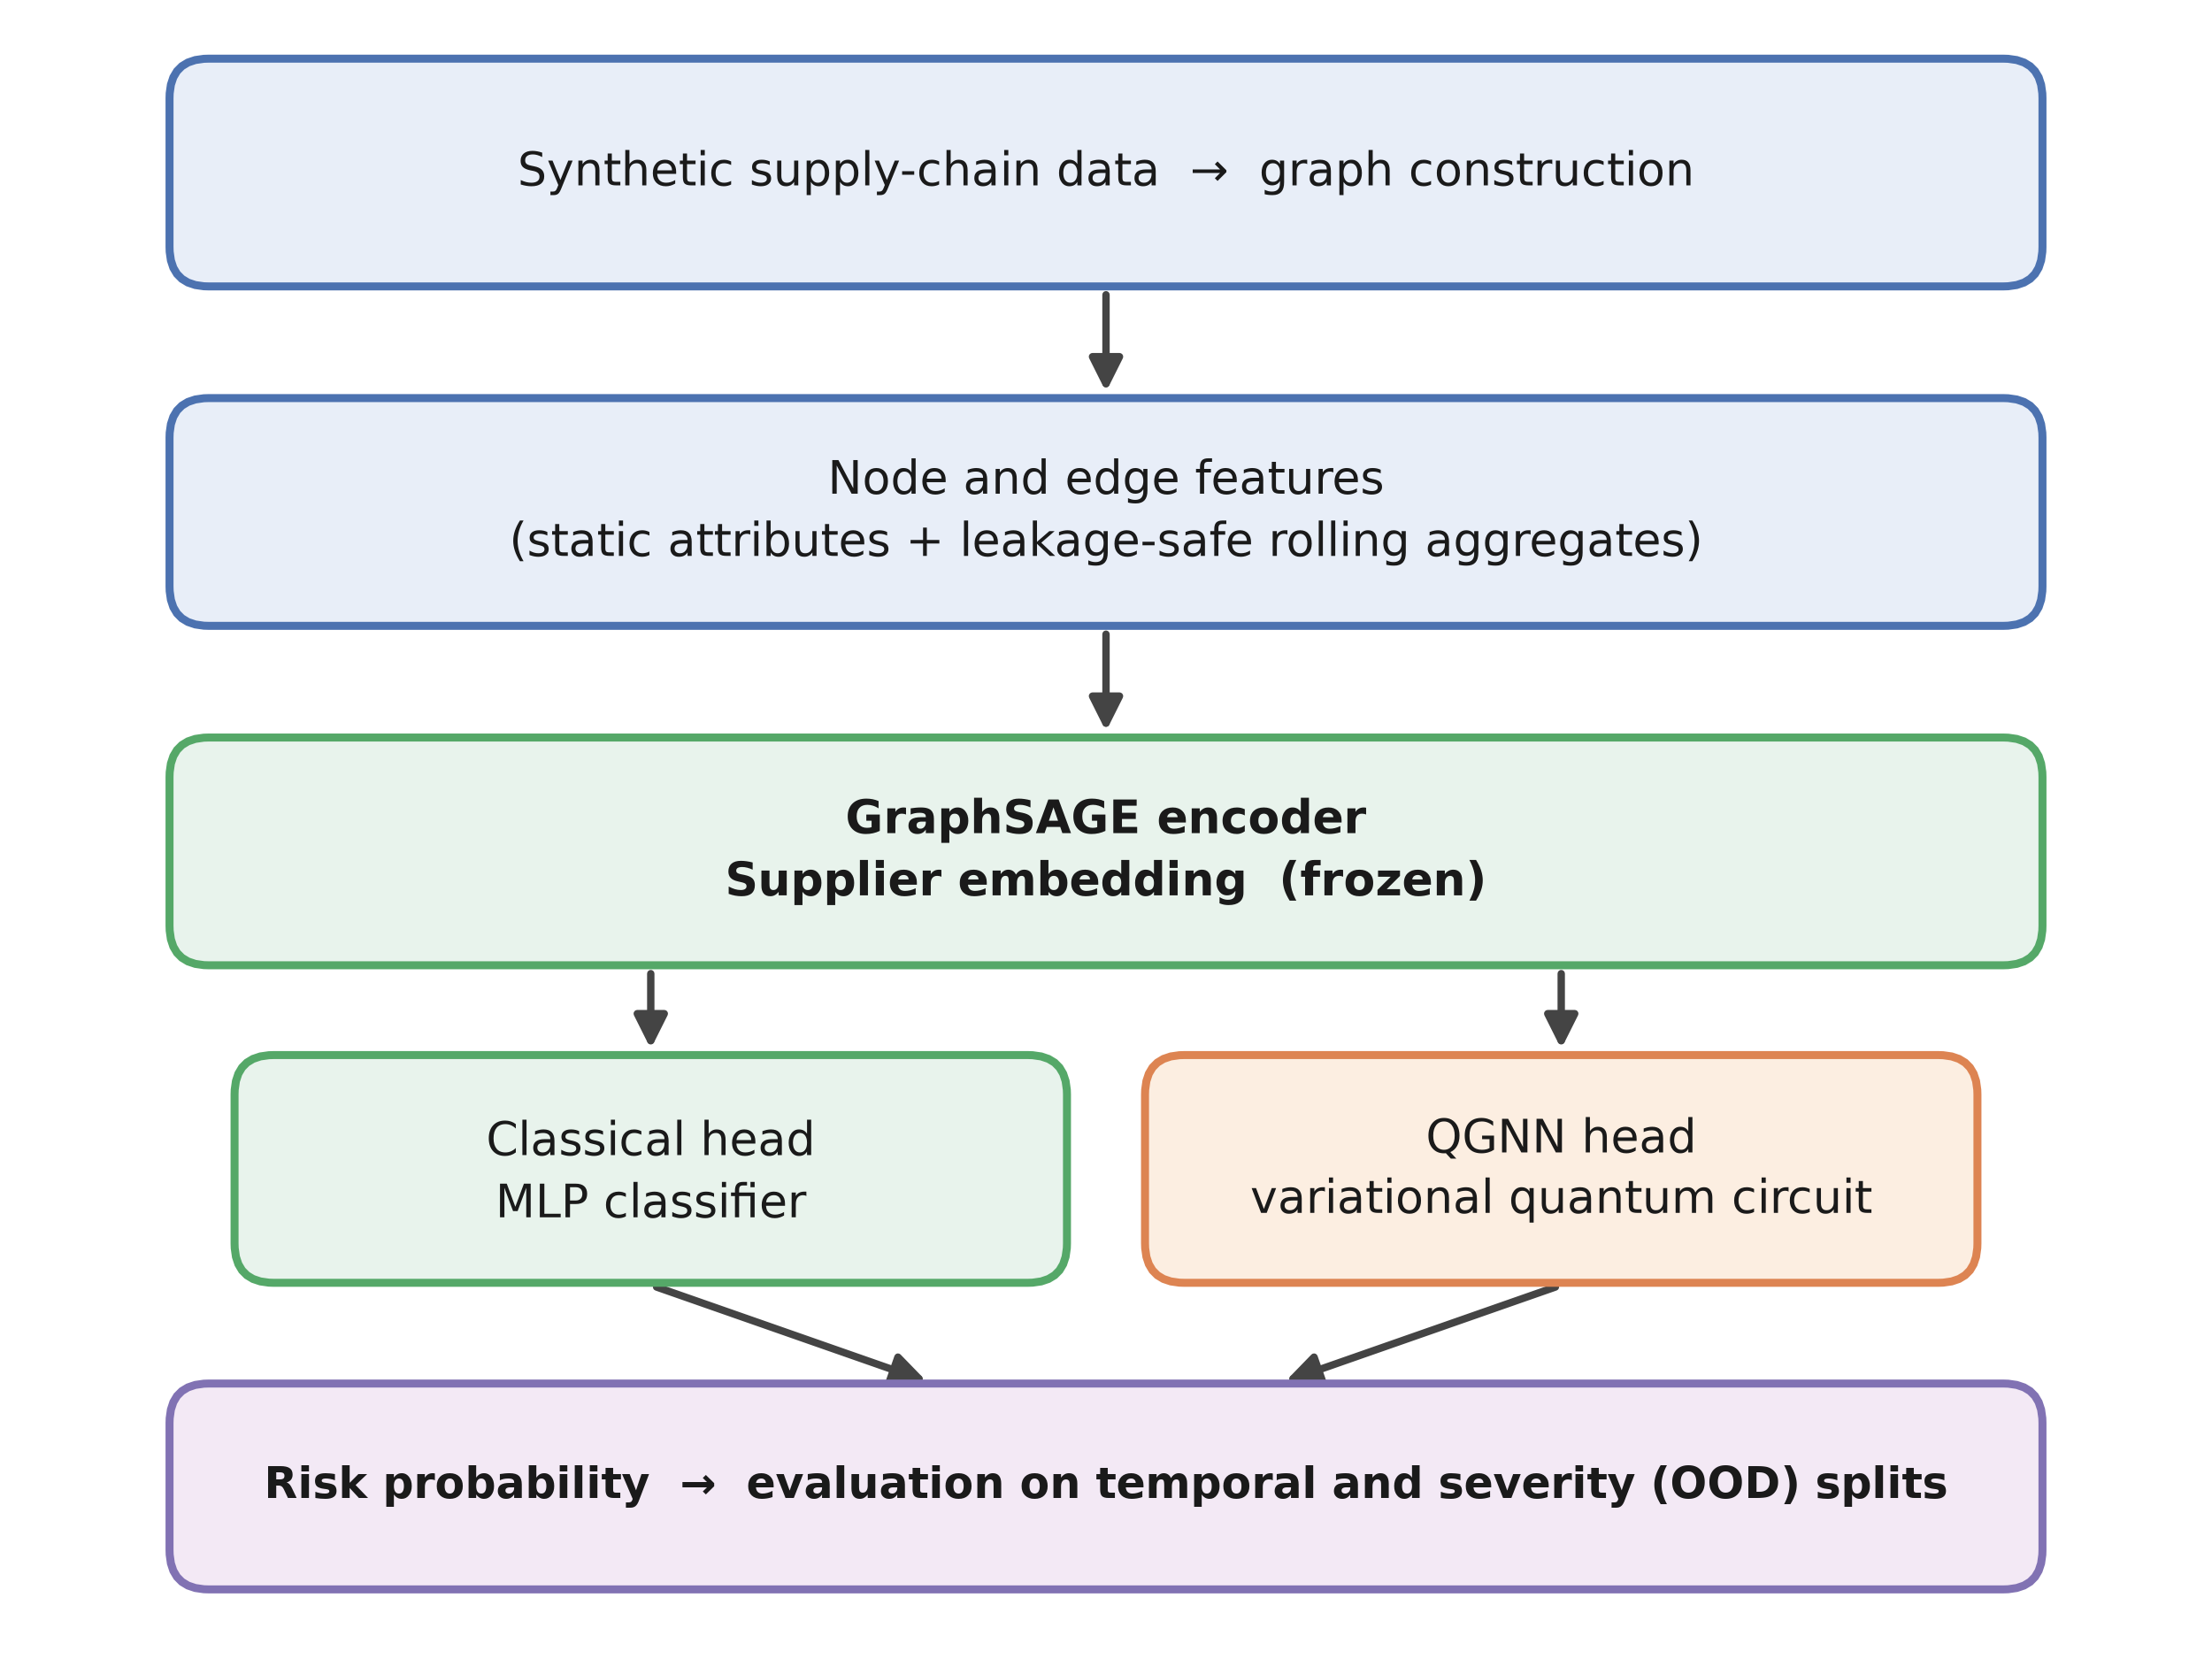
\includegraphics[height=0.80\textheight]{system_diagram.png}
\end{center}
\end{frame}
%--------------------------------------------
%%------------------------------------------------
\section[Future Plan]{Concrete Future Plan}
\begin{frame}[t]
\frametitle{Concrete Future Plan}
\bodyfont
\begin{itemize}
\setlength{\itemsep}{12pt}
  \item \textbf{Benchmark and graph:} Synthetic supply-chain dataset with
        black-swan events; heterogeneous graph construction
  \item \textbf{Classical baseline:} GraphSAGE encoder trained and
        evaluated on temporal and severity splits
  \item \textbf{QGNN baseline:} VQC head on the frozen GraphSAGE
        embedding; training stabilisation (patience, output scaling,
        LayerNorm)
  \item \textbf{Final evaluation:} Classical vs.\ QGNN over multiple
        seeds: ranking, calibration and stability metrics
\end{itemize}
\end{frame}
%----------------------------------------------
%%------------------------------------------

\section{Expected Outcomes}
\begin{frame}[t]
\frametitle{Expected Outcomes}
\bodyfont
\begin{itemize}
\setlength{\itemsep}{12pt}
  \item \textbf{Working classical GraphSAGE baseline and hybrid QGNN} for
        supplier disruption-risk prediction --- both implemented on one
        shared data and training pipeline
  \item \textbf{A controlled comparison of the two models} --- same data,
        splits, metrics and multiple seeds; PR-AUC as primary metric
  \item \textbf{Understanding of normal vs.\ severe-condition behavior} ---
        temporal split and severity (out-of-distribution) split, reported
        separately
  \item \textbf{Clearly scoped conclusions} --- stated for a synthetic
        benchmark on an ideal simulator, not as a general quantum-advantage
        claim
\end{itemize}
\end{frame}
%%---------------------------------------------
%%------------------------------------------------
%%------------------------------------------------
\section{Summary}
\begin{frame}
\frametitle{Summary}
\bodyfont
\begin{itemize}
  \item \textbf{Problem:} supplier procurement risk is a rare-event prediction
        task on a network where disruptions propagate
  \vspace{0.5em}
  \item \textbf{Gap:} supplier-risk studies are classical, and quantum studies
        target other domains such as finance
  \vspace{0.5em}
  \item \textbf{Idea:} pair a classical GraphSAGE encoder with a small
        variational quantum circuit head for supplier risk prediction
  \vspace{0.5em}
  \item \textbf{Approach:} a controlled comparison against a classical GraphSAGE
        baseline, studying which design factors matter
  \vspace{0.5em}
  \item \textbf{Expected contribution:} an evidence-based, clearly scoped
        understanding of when a quantum head helps, not a claim of quantum
        advantage
\end{itemize}
\end{frame}
%-----------------------------------------------

\section[Timeline]{Timeline Chart}
\begin{frame}
\frametitle{Timeline Chart}
\vspace{0.5em}
\begin{center}
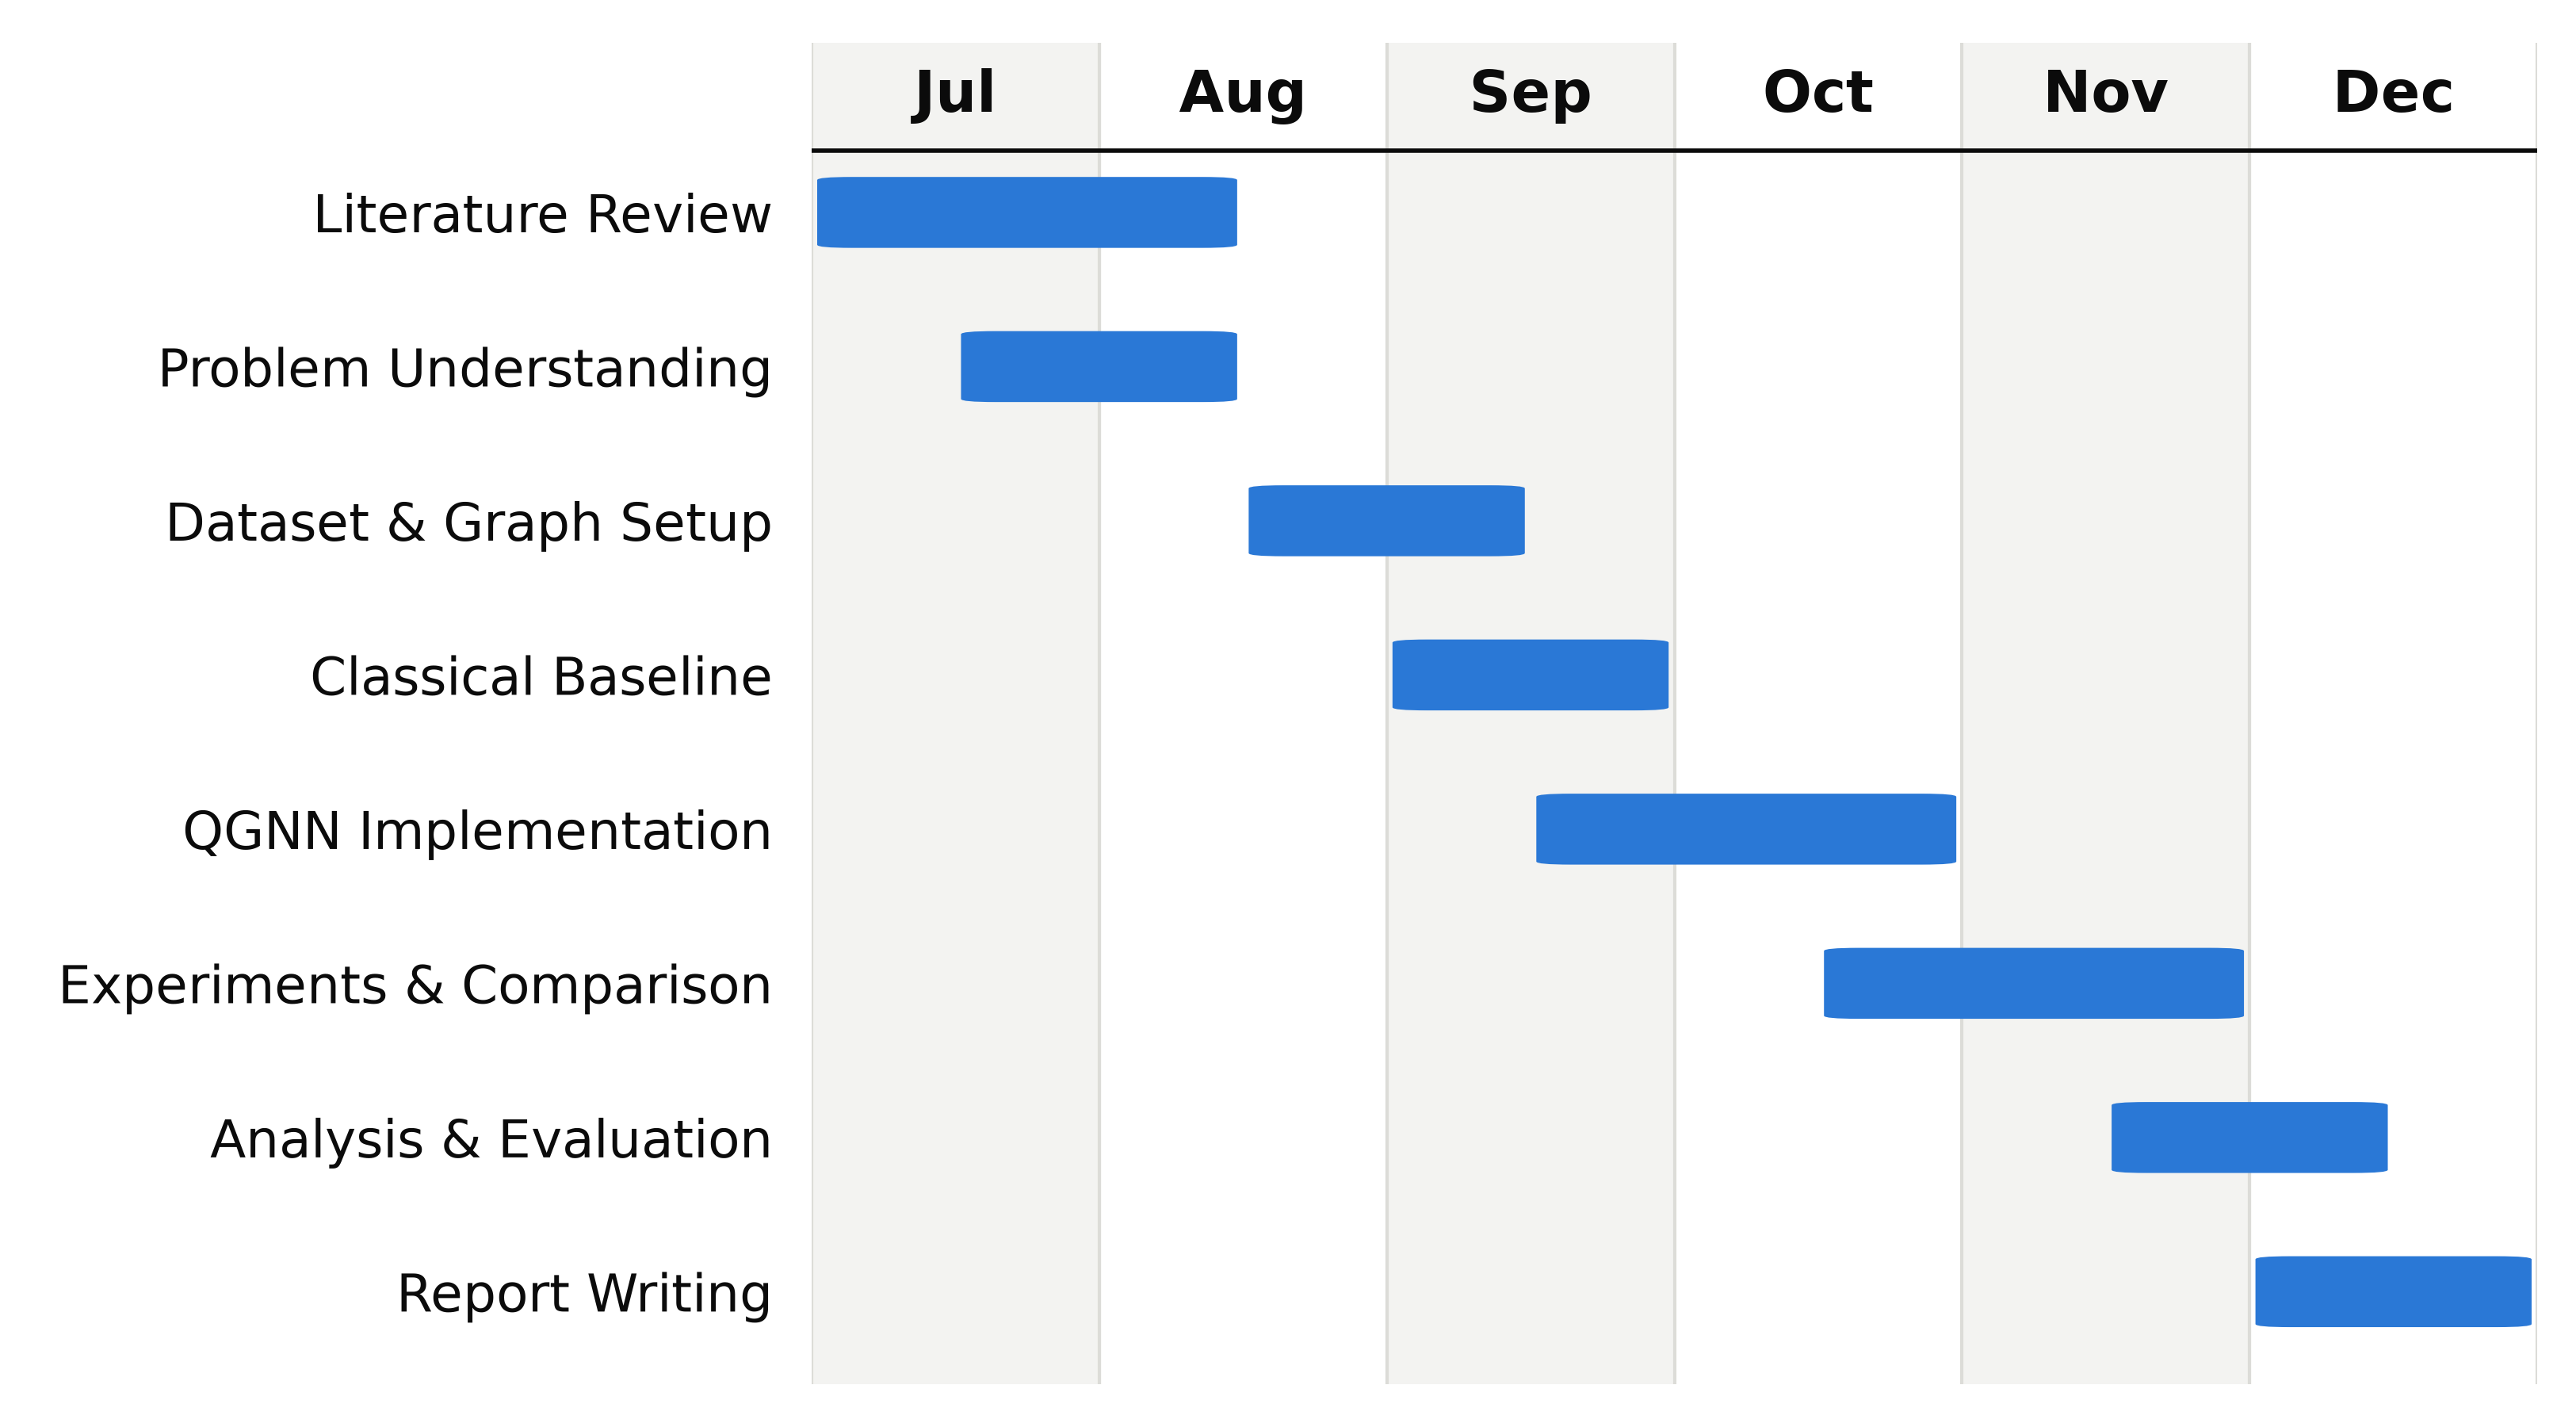
\includegraphics[width=\linewidth]{timeline_gantt.png}
\end{center}
\end{frame}
%------------------------------------------------

\begin{frame}[t]
\frametitle{Timeline Chart Contd...}
\tabfont
\centering
\textbf{Table 6: Project Timeline (July -- December)}\\[0.5em]
\renewcommand{\arraystretch}{1.3}
\begin{tabularx}{\linewidth}{|l|X|}
\hline
\textbf{Month} & \textbf{Planned Work} \\ \hline
\textbf{July -- Aug} & Literature review and problem understanding; defining
the supplier procurement-risk problem and reviewing recent GNN/QGNN
literature \\ \hline
\textbf{September} & Synthetic supply-chain dataset and heterogeneous graph
construction; begin classical GraphSAGE baseline \\ \hline
\textbf{October} & Complete classical GraphSAGE baseline; design and
implement the QGNN --- VQC head on the frozen GraphSAGE embedding, with
training stabilisation (patience, output scaling, LayerNorm) \\ \hline
\textbf{November} & Run experiments comparing classical vs.\ QGNN on
temporal and severity splits; begin analysis and evaluation \\ \hline
\textbf{December} & Complete analysis and evaluation (ranking, calibration,
stability metrics); write the dissertation report \\ \hline
\end{tabularx}
\end{frame}
%-------------------------------------------
%%%------------------------------------------------
\section{References}

% order: the five papers cited on the slides first ([1]-[5]), then the rest of refs.bib
\nocite{fareed2026,ziaria2026,rahman2026,lamichhane2025,larbi2025,innan2024,tudisco2024,soni2024,jiang2022,yadav2021}
\nocite{*}
\setbeamertemplate{bibliography item}[text]
\setbeamercolor{bibliography entry author}{fg=black}
\setbeamercolor{bibliography entry title}{fg=black}
\setbeamercolor{bibliography entry location}{fg=black}
\setbeamercolor{bibliography entry note}{fg=black}
\begin{frame}[t,allowframebreaks=1.0]
\frametitle{References}
\tiny
\setlength{\itemsep}{0pt}\setlength{\parskip}{0pt}
\bibliographystyle{ieeetr}
\bibliography{refs}
\end{frame}

\begin{frame}
\begin{center}
\Huge{\textbf {\textcolor[rgb]{0.6,0.0,0.0}{{Questions/ Discussion}}}}

\end{center}
\end{frame}

\end{document}
